

% In this chapter, we review the literature on techniques for building compact neural networks.
% First of all, we present, in detail, related work which uses tools from linear algebra and structured matrices. 
% Finally, we present in a more concise way concurrent techniques like using specific memory representation or using neural architecture search.
% These techniques are mostly orthogonal to our contributions.


% We have seen in the Introduction (\Cref{chapter:ch2-introduction}) and Background (\Cref{chapter:ch2-background}) that neural networks tend to be over-parametrized which lead to difficult and expensive training and overfitting.


% In this section, we review the literature for building compact neural networks.
% As seen in the Introduction (\Cref{chapter:ch1-introduction}) and Background (\Cref{chapter:ch2-background}), scaling up networks can lead to an increase in accuracy.
% Researchers have demonstrated that increasing the width of shallow neural networks increased their performance~\cite{howard2017mobilenets,sandler2018mobilenetv2,tan2019mnasnet,zagoruyko2016wide} due to their capacity to capture more fine-grained features.
% Increasing depth is a common and effective way to scale neural networks and many deep architectures have been proposed~\cite{he2016deep, huang2016deep, szegedy2016rethinking,szegedy2017inception,xiao2018dynamical}. 
% The intuition is that deep neural network can capture richer and more complex features.


As seen in the Introduction (\Cref{chapter:ch1-introduction}), scaling up networks can lead to better performance.
Increasing the width of shallow neural networks can increase their performance~\cite{howard2017mobilenets,sandler2018mobilenetv2,tan2019mnasnet,zagoruyko2016wide} due to their capacity to capture more fine-grained features.
As well, increasing depth is a common and effective approach to capture richer and more complex features and increase performance, many deep architectures have been proposed~\cite{he2016deep,huang2016deep, szegedy2016rethinking,szegedy2017inception,xiao2018dynamical}.
However, large neural networks lead to difficult and expensive training and overfitting and after observing that a lot of parameters in large neural networks were redundant~\cite{dai2018compressing,frankle2018lottery}, an important question arises: \emph{do neural networks needs to be over-parameterized? And if not, how to build accurate and compact neural networks?} 



% --> Compact Neural Networks Architecture

% Without consideration of specific memory representations, data structures or structured linear layers, it is still possible to design compact neural networks.
%
% However, researchers have demonstrated that increasing the width of shallow neural networks increased their performance~\cite{howard2017mobilenets,sandler2018mobilenetv2,tan2019mnasnet,zagoruyko2016wide} due to their capacity to capture more fine-grained features.
% Finally, depth is a common and effective way to scale neural networks and many deep architectures have been proposed~\cite{he2016deep, huang2016deep, szegedy2016rethinking,szegedy2017inception,xiao2018dynamical}. 
% The intuition is that deep neural network can capture richer and more complex features.
%
% After observing that large and deep neural networks outperformed shallow ones \cite{huang2019gpipe,brown2020language} and the observation that a lot of parameters in large neural networks were redundant~\cite{dai2018compressing,frankle2018lottery}, an important question arises: \emph{do neural networks needs to be large \ie, deep and wide, and if not, which architecture provides the best accuracy?} 

% \citet{ba2014deep} tried to answer this question and empirically demonstrated that shallow neural networks can learn the complex functions previously learned by another neural network. 
% This observation was then leveraged by~\citet{hinton2015distilling} for compressing trained neural networks.
% Their technique, called \emph{model distillation}, consists to train a large complex model using all the available data and resources to be as accurate as possible, then a smaller and more compact model is trained to approximate the first model.
% Although, this approach can be interesting for deployment purposes, it is still required to train one large network and one shallow, which entails a significant training cost.
%
% Instead of compressing the model after the training step, researchers still tried to design architectures that are compact by nature but finding the best trade-off between depth, width and performance has proved to be a tedious work.
% In order to scale the search, recent works have devised algorithms to automatically find the best architecture for a specific use case.
% \citet{zoph2018learning,real2019regularized} have tried to tune the wide and depth of neural network architectures to obtain the best trade-off between efficiency and accuracy but these methods required a lot of manual tuning.
% More recently, with a similar method, \citet{tan2019efficientnet} found a new compound scaling method to uniformly scales network width, depth, and resolution leading to groundbreaking result in terms of efficiency and accuracy.




%%%%%%%%%%%%%%%%%%%%%%%%%%%%%%%%%%%%%%%%%%%%%%%%%%%%%%%%%%%%%%%%%%%%%%%%%%%%%%%%
\subsection{Building Compact Neural Networks with Structured Matrices}
\label{subsection:ch3-building_compact_neural_networks_with_structured_matrices}
%%%%%%%%%%%%%%%%%%%%%%%%%%%%%%%%%%%%%%%%%%%%%%%%%%%%%%%%%%%%%%%%%%%%%%%%%%%%%%%%

% An effective method to build compact neural networks is to constrain the hypothesis space in which the learning algorithm ``chooses'' the predictor.
% As seen in \Cref{chapter:ch2-background}, this constraint is called \emph{inductive bias}. 

% Another way of constraining the weight representation and reduce the memory requirement of neural networks is to impose a \emph{structure} on weight matrices. 

% The idea of building compact neural networks with structured matrices consists of replacing the weight matrices $\Wmat^{(i)}$ with \emph{structured matrices}.

% \todotext{this paragraph makes no sense $\downarrow$}



% A structured matrix is a $n \times n$ matrix whose entries have a formulaic relationship, allowing the matrix to be represented with fewer than $n^2$ parameters.
% The formulaic relationship between entries is an important feature to consider, for example, a sparse matrix has fewer than $n^2$ parameters but does not have a clear relationship between its entries.


An effective method to build compact neural networks is to constrain the hypothesis space on \emph{structured neural networks}. 
The idea of structured neural networks consists of replacing the dense weight matrices with \emph{structured matrices}.
A structured matrix is a $n \times n$ matrix which can be represented with fewer than $n^2$ parameters and where the entries are distributed along specific rules.

% %%%%%%%%%%%%%%%%%%%%%%%%%%%%%%%%%%%%%%%%%%%%%%%%%%%%%%%%%%%%%%%%%%%%%%%%%%%%%%%%
% \subsubsection{Neural networks with Specific Structured Linear Maps}
% \label{subsubsection:ch3-neural_networks_with_specific_structured_linear_maps}
% %%%%%%%%%%%%%%%%%%%%%%%%%%%%%%%%%%%%%%%%%%%%%%%%%%%%%%%%%%%%%%%%%%%%%%%%%%%%%%%%


\drawstar

A classic example of structured matrices are \emph{low-rank} matrices which result from the product of two rectangular matrices.
Let $\Umat \in \Rbb^{n \times r}$ and $\Vmat \in \Rbb^{r \times m}$ with $r \ll \min(m, n)$ then the matrix $\tilde{\Wmat} = \Umat \Vmat$ is low-rank of rank $r$.  
By representing the matrix $\tilde{\Wmat}$ with the low-rank decomposition, we can reduce storage from $mn$ parameters to $(mr + nr)$ parameters and accelerate the matrix-vector product from $\mathcal{O}(mn)$ to $\mathcal{O}(mr + rn)$.
\citet{sainath2013lowrank} were among the first to use low-rank matrices in deep learning contexts followed by the work of~\citet{jaderberg2014speeding,yu2017compressing}.
To enforce the low-rank constraint, reduce storage and computation time, they learned the low-rank decomposition directly, \ie the matrices $\Umat$ and $\Vmat$ instead of $\tilde{\Wmat}$ leading to a neural network layer defined as follows:
\begin{equation}
  \phi^\rho_{\Umat, \Vmat, \bvec} (\xvec) = \rho\left( \Umat \Vmat \xvec + \bvec \right) .
\end{equation}
% By replacing the dense weight matrices $\Wmat^{(i)}$ with the product of two rectangular matrices and learning them instead of the dense matrices, they \emph{impose} on the learning procedure the low-rank constraint.
% We can remark that the matrix resulting from the product of $\Umat^\top \Vmat$ has $m^2$ unique values but can still be represented with only $2nm$ values in memory.
The rank of the low-rank weight matrices becomes a hyper-parameter and governs the trade-off between expressivity (\ie constraint on the hypothesis space) and compactness of the final predictor. 
In the same vein, \citet{novikov2015tensorizing} have proposed to replace the dense weight matrices of fully connected layers by the \emph{Tensor Train decomposition} allowing an important reduction of the number of parameters while preserving the expressive power of the layers.


% Although, less expressive, low-rank matrices offer several advantages: they can be represented in computer memory by their decomposition  
%
% For a neural network $N_\Omega$ parameterized by the set of weight matrices and bias vector $\Omega = \left\{ \left( \Wmat^{(i)}, \bvec^{(i)} \right) \right\}_{i \in [d]}$, they proposed to constraint 
%
% replaced the dense weight matrices $\Wmat^{(i)}$ with a product of two rectangular matrices $\Umat, \Vmat \in \Rbb^{n \times m}$ with $n < m$ which led to neural network layer defined as follows:

% In linear algebra, many structures have been discovered and studied~\cite{pan2001structured}. 
% for example, circulant matrices have been used to efficiently solve linear systems~\cite{golub1996matrix} and years later 
% This effectively replaces the complex transform modeled by the fully connected layer by a simple dimensionality reduction.
% Indeed, the last 3 fully connected layers of the AlexNet~\cite{krizhevsky2012imagenet} architecture use 58M out of the 62M total trainable parameters ($> 90\%$ of the total number of parameters).

% comes from the observation that a neural network layer can be seen as dimensionality reduction layer.

\drawstar

A variety of structured matrices have been used to build compact neural networks.
For example, \citet{cheng2015exploration} had the idea to replace the weight matrix of a fully connected layer by the product of a circulant and diagonal matrices where the circulant matrix is learned by a gradient-based optimization algorithm and the diagonal matrix entries are sampled at random in $\{-1, 1\}$ leading the layer to be parameterized by only $n$ values instead of $n^2$ and the matrix-vector product to be efficiently computed with the Fast Fourier Transform and the \Cref{algorithm:ch2-matrix_vector_product_circulant_matrix}.
Despite the reduction of expressivity, their experiments demonstrated good accuracy using only a fraction of the original size of the network (90\% reduction).
The idea of using circulant matrices and other types of structured matrices in neural networks is motivated by the celebrated \citeauthor{johnson1984extensions} lemma which states that a set of points in a high-dimensional space can be embedded into a space of much lower dimension with near preservation of distance between the points.
This result can be formalized as follows:
\begin{lemma}[\citet{johnson1984extensions}]
  Let $\mathcal{X} \subset \Rbb^n$ be a set of $m$ vectors, then for any $0 < \epsilon < \frac{1}{2}$, there exists a map $f: \mathcal{X} \rightarrow \Rbb^k$ for some $k = \mathcal{O}(\epsilon^{-2} \log m)$ such that
  \begin{equation}
    \forall \xvec, \yvec \in \mathcal{X}, \quad (1 - \epsilon) \norm{\xvec - \yvec}_2^2 \leq \norm{f(\xvec) - f(\yvec)}_2^2 \leq (1 - \epsilon) \norm{\xvec - \yvec}_2^2 
  \end{equation}
\end{lemma}
\noindent
More practically, \citet{hinrichs2011johnson} have shown that the \DC transform $\xvec \mapsto \Dmat \Cmat \xvec$, where the matrix $\Dmat$ is a diagonal matrix with entries sampled from $\{1, -1\}$ and $\Cmat$ is a circulant matrix based on a sequence of independent identically distributed random variables respect the \citeauthor{johnson1984extensions} lemma.
Although \citet{cheng2015exploration} used \emph{learned} circulant matrices, therefore relaxing the theoretical guarantee of \citet{hinrichs2011johnson} they showed good empirical results. 

Several transform with structured matrices have been proposed.
The Fastfood transform~\cite{le2013fastfood}, which was originally used for approximating kernel expansions, was later used in neural networks by~\citet{yang2015deep} leading to the Deep Fried Convnets architecture.
The authors have replaced dense matrices of fully connected layers with adaptive structured matrices of the form: $\Smat\Hmat\Gmat\mathbf{\Pi}\Hmat\Bmat$ where $\Smat$, $\Gmat$, and $\Bmat$ are adaptive diagonal matrices, $\mathbf{\Pi}$ is a random permutation matrix, and $\Hmat$ is the Walsh-Hadamard matrix.
Later, the \emph{Structured Spinners} transform of the form: $\Hmat\Dmat^{(3)} \Hmat\Dmat^{(2)} \Hmat\Dmat^{(1)}$, where $\Hmat$ is the Walsh-Hadamard matrix, and $\Dmat^{(i)}$ for $i \in {1, 2, 3}$ is a random $\pm1$-diagonal matrix, was originally proposed by~\citet{andoni2015practical} and used in deep learning settings by~\citet{bojarski2017structured}.

\citet{moczulski2016acdc} build upon the work of~\citet{cheng2015exploration} and \citet{huhtanen2015factoring} and introduced two \emph{Structured Efficient Linear Layers} (SELL) based on the Fourier and cosine transform.
First, by observing that the \DC transform cannot express an arbitrary linear operator they propose to apply the result of \citet{huhtanen2015factoring} which states that almost all matrices can be decomposed as a product of \DC transform.
More formally, 
\begin{theorem}[Reformulation from \citet{huhtanen2015factoring}]
  For every matrix $\Mmat \in \Cnn$, for any $\epsilon > 0$, there exists a sequence of matrices $\Amat^{(1)} \ldots \Amat^{(2n-1)}$ where $\Amat^{(i)}$ is a circulant matrix if $i$ is odd, and a diagonal matrix otherwise, such that $\norm{\Amat^{(1)} \ldots \Amat^{(2n-1)} - \Mmat} < \epsilon$.
  \label{theorem:ch3-huhtanen}
\end{theorem}
\noindent
Based on this result, they proposed the following structured layer:
\begin{equation}
  \Phi^\rho_{\Dmat, \Cmat, \bvec} (\xvec) = \rho \left( \left(\prod_{i = 1}^{k} \Dmat^{(i)} \Cmat^{(i)} \right) \xvec + \bvec \right)
\end{equation}
where $\Dmat$ and $\Cmat$ are sequences of $k$ diagonal and circulant matrices respectively.
This structured is therefore parameterized by $n(2k+1)$ values and the value $k$ becomes an hyper-parameter controlling the trade-off between compactness and expressivity. 
The linear layer can be efficiently computed with the fast Fourier transform and the diagonalization of the circulant matrix. 
Recall that if the circulant matrix $\Cmat^{(i)} =  \circulant\left(\cvec^{(i)}\right)$ where $\cvec^{(i)}$ is the vector characteristic then we can express the circulant matrix $\Cmat^{(i)}$ as follows: $\Cmat^{(i)} = \frac{1}{n} \Umat_n^* \diag(\Umat_n \cvec^{(i)}) \Umat_n$.
% \begin{equation}
%   \Cmat^{(i)} = \frac{1}{n} \Umat_n^* \diag(\Umat_n \cvec^{(i)}) \Umat_n \enspace.
% \end{equation}
The structured layer can then be written as the following:
\begin{equation}
  \Phi^\rho_{\dvec, \cvec, \bvec} (\xvec) = \rho \left(\frac{1}{n^k} \left(\prod_{i = 1}^{k} \diag\left(\dvec^{(i)}\right) \Umat_n^* \diag\left(\Umat_n \cvec^{(i)}\right) \Umat_n \right) \xvec + \bvec \right)
\end{equation}
\noindent
Although interesting and demonstrating good empirical results, their work suffers form from multiple limitations. 
First, the result of~\citet{huhtanen2015factoring} is expressed with respect to $n$, the size of the matrices $\Amat$.
Therefore, the theorem does not provide any insights regarding the expressive power of $k$ factors when $k$ is much lower than $2n-1$ as it is the case in most practical scenarios they consider.
Finally, for practical reasons, they replaced the Fourier transform with the cosine transform.
As far as we can tell, the theoretical guarantees available with the Fourier Transform do not apply to the cosine transform because the cosine transform does not diagonalize circulant matrices \cite{sanchez1995diagonalizing}.



\begin{figure}[t]
   \centering
   \begin{subfigure}[b]{0.32\textwidth}
       \centering
       \begin{equation*}
	  \leftmatrix
	    \tvec_0      & \tvec_1 & \cdots     & \tvec_{n-1} \\
	    \tvec_{-1}   & \tvec_0 & \ddots     & \vdots      \\
	    \vdots       & \ddots  & \ddots     & \tvec_1     \\
	    \tvec_{-n+1} & \cdots  & \tvec_{-1} & \tvec_0
	  \rightmatrix
       \end{equation*}
       \caption*{Toeplitz}
   \end{subfigure}
   \hfill
   \begin{subfigure}[b]{0.32\textwidth}
       \centering
       \begin{equation*}
	  \leftmatrix
	    1 & \vvec_0     & \cdots & \vvec_0^{n-1} \\
	    1 & \vvec_1     & \cdots & \vvec_1^{n-1} \\
	    1 & \vdots      &        & \vdots        \\
	    1 & \vvec_{n-1} & \cdots & \vvec_{n-1}^{n-1}
	  \rightmatrix
       \end{equation*}
       \caption*{Vandermonde}
   \end{subfigure}
   \hfill
   \begin{subfigure}[b]{0.32\textwidth}
       \centering
       \begin{equation*}
	  \leftmatrix
	  \frac{1}{\uvec_0 - \vvec_{0}}     & \cdots & \frac{1}{\uvec_0 - \vvec_{n-1}} \\
	  \frac{1}{\uvec_1 - \vvec_{0}}     & \cdots & \frac{1}{\uvec_1 - \vvec_{n-1}} \\
	  \vdots                            & \cdots & \vdots                          \\
	  \frac{1}{\uvec_{n-1} - \vvec_{0}} & \cdots & \frac{1}{\uvec_{n-1} - \vvec_{n-1}}
	  \rightmatrix
       \end{equation*}
       \caption*{Cauchy}
   \end{subfigure}
   \caption{Representation of Toeplitz, Vandermonde and Cauchy matrices}
  \label{figure:ch3-example_structure_matrices}
\end{figure}


\drawstar

% %%%%%%%%%%%%%%%%%%%%%%%%%%%%%%%%%%%%%%%%%%%%%%%%%%%%%%%%%%%%%%%%%%%%%%%%%%%%%%%%
% \subsubsection{General Representation of Structured Linear Maps: LDR and K-Matrices}
% \label{subsubsection:ch2-general_representation_of_structured_linear_maps:_ldr_and_k-matrices}
% %%%%%%%%%%%%%%%%%%%%%%%%%%%%%%%%%%%%%%%%%%%%%%%%%%%%%%%%%%%%%%%%%%%%%%%%%%%%%%%%


Other types of structured matrices that reduce the memory footprint but also accelerate the matrix-vector product have been used to build compact neural networks.
Bellow a description of known matrix structured:
\begin{itemize}
  \item \textbf{Toeplitz matrix}: As seen in \Cref{subsection:ch2-toeplitz_matrices}, a Toeplitz matrix, named after Otto Toeplitz, has constant values along each of their diagonals. When the matrix as the same property for anti-diagonals, the matrix is a \emph{Hankel matrix}.
  % \item \textbf{Block Circulant matrix}: A block circulant matrix is a matrix in which each block is repeated identically along diagonals (like block Toeplitz matrices) and each ``row of blocks'' is cyclic right shift of the previous one.
  \item \textbf{Vandermonde matrix}: A Vandermonde matrix, named after Alexandre-Théophile Vandermonde, is a matrix with the terms of a geometric progression in each row.  
    A very important special case is the complex matrix associated with the Discrete Fourier transform (DFT) presented in \Cref{definition:ch2-fourier_matrix} which has Vandermonde structure.
  \item \textbf{Cauchy matrix}: A Cauchy matrix, named after Augustin Louis Cauchy, is a $m \times n$ matrix with elements $a_{ij}$ such that $a_{ij} = (\uvec_i - \vvec_j)^{-1}$ with $\uvec_i - \vvec_j \neq 0$, $i \in \{0,\dots,m-1\}$ and $j \in \{0,\dots,n-1\}$.
\end{itemize}
\Cref{figure:ch3-example_structure_matrices} shows the representation of the parameters sharing of Toeplitz, Vandermonde and Cauchy matrices.
These matrices can be unified into a framework with the notion of \emph{Low Displacement Rank} (LDR).
Each of these matrices can be associated with a displacement operator $\Rmat: \Rbb^{m \times n} \rightarrow \Rbb^{m \times n}$ which takes a matrix, $\Mmat$, and outputs a low rank matrices such that $\rank(\Rmat(\Mmat)) \ll \min(m,n)$.
This displacement rank approach has been initially proposed by~\citet{kailath1979displacement} and have been further studied by~\citet{kailath1995displacement,pan2001structured}. 
More formally, we can define two displacement operators (for simplification, we consider $m = n$):
\begin{definition}[\emph{Sylvester} \& \emph{Stein} displacement operators]
  Let $\Amat, \Bmat \in \Rbb^{n \times n}$, the \emph{Sylvester} displacement operator denoted $\Rmat = \triangleopdown_{\Amat, \Bmat}: \Rbb^{n \times n} \rightarrow \Rbb^{n \times n}$ is defined as follows:
  \begin{equation}
    \triangleopdown_{\Amat, \Bmat} (\Mmat) \triangleq \Amat \Mmat - \Mmat \Bmat
  \end{equation}
  The \emph{Stein} displacement operator denoted $\Rmat = \triangleopup_{\Amat, \Bmat}: \Rbb^{n \times n} \rightarrow \Rbb^{n \times n}$ is defined as follows:
  \begin{equation}
    \triangleopup_{\Amat, \Bmat} (\Mmat) \triangleq \Mmat - \Amat \Mmat \Bmat
  \end{equation}
  where $\triangleopdown_{\Amat, \Bmat} = \Amat \triangleopup_{\Amat^{-1}, \Bmat}$ if the operator matrix $\Amat$ is non-singular, and $\triangleopdown_{\Amat, \Bmat} = -\triangleopup_{\Amat, \Bmat^{-1}}$ if the operator matrix $\Bmat$ is non-singular.
\end{definition}
\begin{table}[t]
  \centering
  {\small
  \begin{tabular}{c|c|c|c}
    \toprule
    \multicolumn{2}{c|}{\textbf{Operator Matrices}} & \textbf{Class of structured} & \textbf{Rank of } \\
    \textbf{A} & \textbf{B} & \textbf{matrices M} & $\triangleopdown_{\Amat, \Bmat}(\Mmat)$ \\
    \midrule
    $\Zmat_1$                & $\Zmat_0$                & Toeplitz               & $\leq 2$ \\
    $\Zmat_1$                & $\Zmat_0^\top$           & Hankel                 & $\leq 2$ \\
    $\Zmat_0 + \Zmat_0^\top$ & $\Zmat_0 + \Zmat_0^\top$ & Toeplitz + Hankel      & $\leq 4$ \\
    $\diag(\vvec)$           & $\Zmat_0$                & Vandermonde            & $\leq 1$ \\
    $\Zmat_0$                & $\diag(\vvec)$           & Inverse of Vandermonde & $\leq 1$ \\
    $\diag(\uvec)$           & $\diag(\vvec)$           & Cauchy                 & $\leq 1$ \\
    $\diag(\vvec)$           & $\diag(\uvec)$           & Inverse of Cauchy      & $\leq 1$ \\
    \bottomrule
  \end{tabular}
  }
  \caption{Displacing Matrices Associated with Families of Structured Matrices \cite{pan2001structured}}
  \label{table:ch2-displacing_matrices}
  \vspace{0.5cm}
\end{table}

\noindent
Based on this definition, we can then say that, if $\Mmat$ is Toeplitz, it exists operator matrices $\Amat$ and $\Bmat$ such that $\triangleopdown_{\Amat, \Bmat} (\Mmat)$ or $\triangleopup_{\Amat, \Bmat} (\Mmat)$ is low rank.
In particular, $\Amat$ and $\Bmat$ can be chosen to be diagonal or $f$-unit-circulant matrices (\eg \Cref{definition:ch2-f_circulant_matrix}) for several classes of structured matrices.
\Cref{table:ch2-displacing_matrices} shows some specific choices of operators for the four basic classes of structured matrices and for some related matrices.
An important result allows us to express structured matrices with low-displacement rank directly as a function of its low displacement generators.  
For the Stein type displacement operator, we have the following result:
\begin{theorem}[Krylov Decomposition~\citet{pan2003inversion,sindhwani2015structured}]
  If an $n \times n$ matrix $\Mmat$ is such that $\triangleopup_{\Amat, \Bmat}(\Mmat) = \Gmat \Hmat^\top$ where 
  $\Gmat = (\gvec^{(1)} \ldots \gvec^{(r)}), \Hmat = (\hvec^{(1)} \ldots \hvec^{(r)}) \in \Rbb^{n \times r}$ 
  and the operator matrices satisfy: $\Amat^n = a \Imat$, $\Bmat^n = b \Imat$ for some scalars $a, b$, then $\Mmat$ can be expressed as: 
  \begin{equation}
    \Mmat = \frac{1}{1 - ab} \sum_{j=1}^{r} ~\krylov(\Amat, \gvec^{(j)}) ~\krylov(\Bmat^\top, \hvec^{(j)})^\top
    \label{equation:ch3-krylov_decomposition}
  \end{equation}
  where $\krylov(\Amat, \vvec)$ is defined by:
  \begin{equation}
    \krylov(\Amat, \vvec) = [\vvec~~\Amat\vvec~~\Amat^2 \vvec \ldots \Amat^{n-1} \vvec]
  \end{equation}
  \label{theorem:ch3-krylov_decomposition}
\end{theorem} 
\noindent
This theorem can be simplified for \emph{Toeplitz-like matrices} as follows:
\begin{theorem}[Toeplitz-like matrix decomposition \citet{pan2001structured}]
  If an $n \times n$ matrix $\Mmat$ satisfies $\triangleopdown_{\Cmat_1, \Cmat_{-1}}(\Mmat) = \Gmat \Hmat^T$ ($\Mmat$ is Toeplitz-like) where $\Gmat = (\gvec ^{(1)} \ldots \gvec^{(r)}], \Hmat = (\hvec^{(1)} \ldots \hvec^{(r)}) \in \Rbb^{n \times r}$, then $\Mmat$ can be written as: 
  \begin{equation} 
    \Mmat = \frac{1}{2} \sum_{j=1}^{r} \Cmat_1(\gvec^{(j)}) \Cmat_{-1}(\Jmat_n \hvec^{(j)})
    \label{equation:ch3-toeplitz_like_matrix_decomposition}
  \end{equation}
  where $\Jmat_n$ is the reflection matrix of size $n \times n$.
\end{theorem}
\noindent
\citet{sindhwani2015structured} have used this theorem in the context of deep learning.
More precisely, they proposed to parameterized neural networks layers as in \Cref{equation:ch3-toeplitz_like_matrix_decomposition} and learn the displacement factors $\Gmat$, $\Hmat$ by gradient descent. 
For some $\Gmat = \leftmat \gvec^{(1)} \ldots \gvec^{(r)} \rightmat, \Hmat = \leftmat \hvec^{(1)} \ldots \hvec^{(r)} \rightmat \in \Rbb^{n \times r}$, their layer is defined as follows:
\begin{equation}
  \Phi^\rho_{\Gmat, \Hmat, \bvec}(\xvec) = \rho\left( \left(\sum_{j=1}^{r} \Cmat_1\left(\gvec^{(j)}\right) \Cmat_{-1}\left(\Jmat_n \hvec^{(j)}\right) \right) \xvec + \bvec \right)
\end{equation}
\noindent
They also show that this class of layer are very rich of a modeling perspective:
\begin{theorem}[LDR expressivity \citet{pan2001structured,sindhwani2015structured}] ~\\
  The set of all $n \times n$ matrices that can be written as, $\sum_{i=1}^{r} \Cmat_1(\gvec^{(i)}) \Cmat_{-1}(\hvec^{(i)})$
  for some $\Gmat = \leftmat \gvec^{(1)} \ldots \gvec^{(r)} \rightmat,
  \Hmat = \leftmat \hvec^{(1)} \ldots \hvec^{(r)} \rightmat \in \Rbb^{n \times r}$ contains:
  \begin{compactitem}
    \item All $n \times n$ Circulant and Skew-Circulant matrices for $r \geq 1$.
    \item All $n \times n$ Toeplitz matrices for $r \geq 2$.
    \item Inverses of Toeplitz matrices for $r \geq 2$.
    \item All products of the form $\Amat^{(1)} \ldots \Amat^{(t)}$ for $r \geq 2t$.
    \item All linear combinations of the form $\sum_{i=1}^p \beta_i \Amat^{(1, i)} \ldots \Amat^{(t, i)}$ where $r \geq 2tp$.
    \item All $n\times n$ matrices for $r=n$.
  \end{compactitem}
  where each $\Amat^{(i)}$ above is a Toeplitz matrix or the inverse of a Toeplitz matrix. 
\end{theorem}
\noindent
In the same line of work, \citet{thomas2018learning} have proposed neural network layers directly form \Cref{equation:ch3-krylov_decomposition} which encompasses an even larger family of structured matrices including Toeplitz-like, Vandermonde-like, Cauchy-like.
Despite being elegant and general, we found that the LDR framework suffers from several limits which are inherent to its generality and makes it difficult to use in the context of large and deep neural networks.
First, the training procedure for learning LDR matrices is highly involved and implies many complex mathematical objects such as Krylov matrices.
Then, as acknowledged by the authors, the number of parameters required to represent a given structured matrix (a Toeplitz matrix) in practice is unnecessarily high (higher than required in theory). 

\drawstar

More recently, another type of generalization of structured linear maps has been proposed by~\citet{dao2020kaleidoscope} and used in the context of deep neural networks.
They introduced a family of matrices called \emph{kaleidoscope matrices} (K-matrices) that capture any sparse matrix with near-optimal space (parameter) and time (arithmetic operation) complexity.
More precisely, their representation is based on products of a particular building block known as a butterfly matrix~\cite{parker1995random,dao2019learning}.





%%%%%%%%%%%%%%%%%%%%%%%%%%%%%%%%%%%%%%%%%%%%%%%%%%%%%%%%%%%%%%%%%%%%%%%%%%%%%%%%
\subsection{Other Approaches for Building Compact Neural Networks}
\label{subsection:ch3-other_approaches_for_building_compact_neural_networks}
%%%%%%%%%%%%%%%%%%%%%%%%%%%%%%%%%%%%%%%%%%%%%%%%%%%%%%%%%%%%%%%%%%%%%%%%%%%%%%%%


Numerous other directions have been investigated to build compact and cost-effective neural networks, for example \citet{gupta2015deep,micikevicius2018mixed} have proposed to represent weights with limited numerical precision to reduce training time and memory requirements.
They used half-precision floating-point format instead of single-precision floating-point format which uses 32 bits of computer memory.
In the same direction, \citet{courbariaux2015binaryconnect} have proposed a method to train neural networks with binary weights.

An important idea in model compression proposed by~\citet{bucilua2006model}, is based on the observation that the model used for training is not required to be the same as the one used for inference, indeed, compressed models after training can be deployed on smartphones or IoT devices.
Based on this idea, multiple post-processing techniques have been developed: a quantization procedure which consists in converting the weights into a binary or integer formats \emph{after} the training phase~\cite{mellempudi2017ternary,rastegariECCV16}, pruning techniques~\cite{dai2018compressing,han2015deep,lin2017runtime} or sparsity regularizers~\cite{collins2014memory,dai2018compressing,liu2015sparse} which consists in removing redundant weights after training and taking advantage of the sparse structure of the weight matrices.

Sparse neural networks have also been extensively studied since the seminal paper of \citet{frankle2018lottery} in which he proposes the \emph{Lottery Ticket Hypothesis}. 
This hypothesis states that it exists a sparse subnetwork of dense neural network that when trained in isolation can match the test accuracy of the original dense network after training for at most the same number of iterations. 
This hypothesis led to a series of works on sparse neural networks \cite{zhou2019deconstructing,malach2019proving,evci2020rigging}.

Moreover, \citet{ba2014deep} have empirically demonstrated that shallow neural networks can learn the complex functions previously learned by another deep neural networks.
This result led \citet{hinton2015distilling} to propose a technique called \emph{model distillation} which consists in training a large complex model using all the available data and resources to be as accurate as possible, then a smaller and more compact model is trained to approximate the first model.
Although interesting for deployment purposes, this approach still requires to train one large network and one shallow, which entails a significant training cost.

\begin{figure}[t]
  \centering
  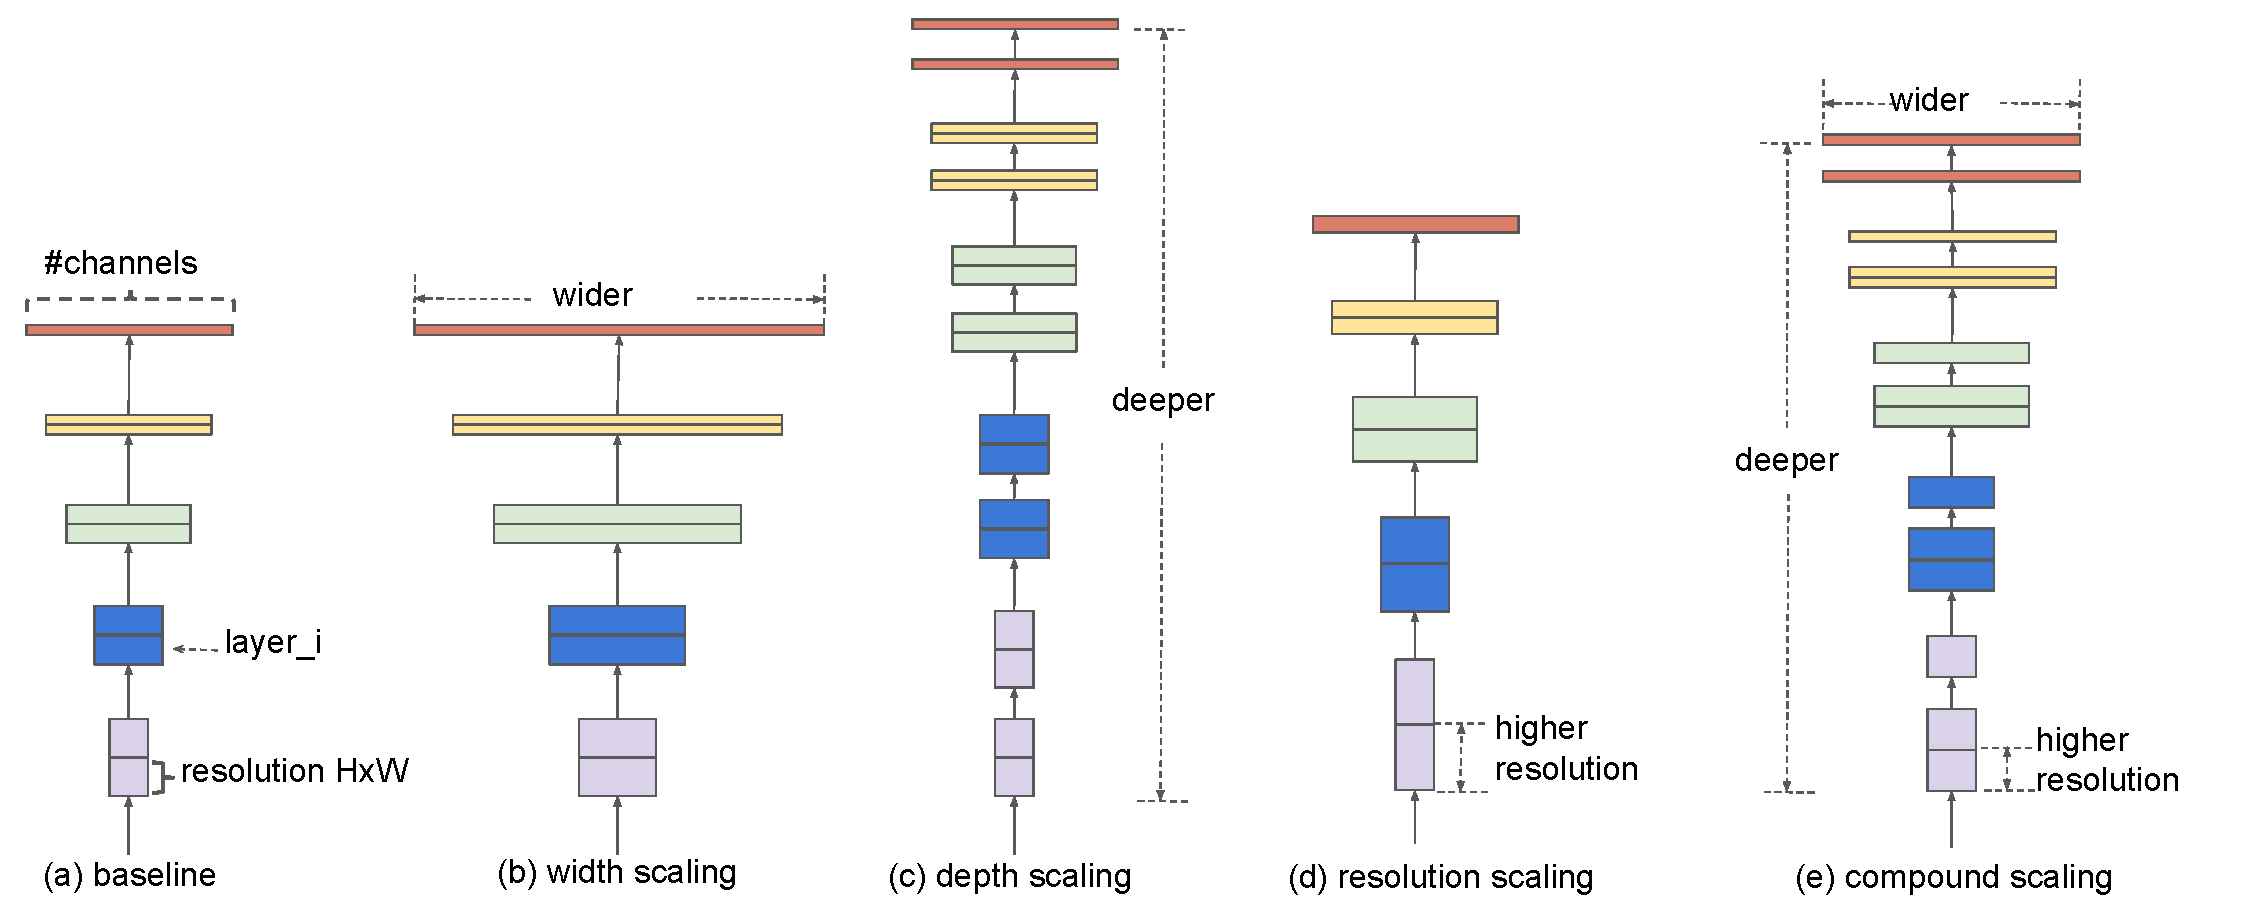
\includegraphics[width=0.80\textwidth]{figures/main/ch3-related_work/scalecompare.pdf}
  \caption{Illustration of the scaling of the EfficientNet architecture \cite{tan2019efficientnet}.}
  \label{figure:p1-ch3-illustration_efficientnet}
\end{figure}

More recently, \citet{zoph2018learning,real2019regularized} have designed algorithms that automatically tune the width and depth of neural network architectures to obtain the best trade-off between compactness and accuracy.
With this approach, \citet{tan2019efficientnet} found a new compound scaling method that uniformly scales network width and depth leading to efficient and compact architectures.
\Cref{figure:p1-ch3-illustration_efficientnet} illustrate the different scaling proposed by~\citet{tan2019efficientnet}.


% Finally, in the context of deep learning, compact representations have gained much attention over the past years as a way to compress models or to reduce memory requirements.
% In this thesis, we focus on building compact neural networks with structured matrices.
% Hereafter, we present a comprehensive overview of the existing techniques in this line of research.















% \todotext{observation that Hadamard matrices when combined with diagonal Gaussian matrices exhibit properties similar to dense Gaussian random matrices. Yet unlike the latter, Hadamard and diagonal matrices are inexpensive to multiply and store}
%
% This result have led to multiple \emph{Fast Johnson-Lindenstrauss Transform} to embed high-dimensional vectors into lower dimensional space with fast algorithm with reduce memory requirement and fast matrix-vector products.
% For example, \citet{ailon2009fast} have proposed the PHD transorm: $\yvec = \Pmat \Hmat \Dmat \xvec$, where $\Pmat$ is a sparse random matrix with Gaussian entries $\Hmat$ is a 
% Hadamard matrix and $\Dmat$ is a diagonal matrix with $\{1, -1\}$ entries drawn independently with probability $1/2$.

% Another fast transform have been proposed involving circulant matrices.
% Recall from \Cref{subsection:ch2-circulant_matrices} that circulant matrices are a special case of Toeplitz matrices, they have constant values along each of their diagonals but also exhibit a circulant pattern where each row of a circulant matrix is a cyclic right shift of the previous one. 


% that circulant, which have been used to perform dimensionality reduction~\cite{hinrichs2011johnson,vybiral2011variant}, binary embedding~\cite{yu2014circulant} and kernel approximation~\cite{yu2015compact} in the context of pattern recognition and machine learning 

% A variety of structured matrices have been used to build compact neural networks.

% circulant matrices are used to perform dimensionality reduction~\cite{hinrichs2011johnson,vybiral2011variant}, binary embedding~\cite{yu2014circulant} and kernel approximation~\cite{yu2015compact} in the context of pattern recognition and machine learning.


% CirCNN: Accelerating and Compressing Deep Neural Networks Using Block-Circulant Weight Matrices
% \cite{ding2017circnn}
%
% Accelerating Deep Neural Networks by Combining Block-Circulant Matrices and Low-Precision Weights
% \cite{qin2019accelerating}
%
% Exploring GPU acceleration of Deep Neural Networks using Block Circulant Matrices
% \cite{dong2020exploring}
%
% Energy-efficient, high-performance, highly-compressed deep neural network design using block-circulant matrices
% \cite{liao2017energy}
%
% CircConv: A Structured Convolution with Low Complexity
% \cite{liao2019circconv}


% \todo{transition}
% -> \cite{ding2017circnn,qin2019accelerating,dong2020exploring,liao2017energy,liao2019circconv}























%%%%%%%%%%%%%%%%%%%%%%%%%%%%%%%%%%%%%%%%%%%%%%%%%%%%%%%%%%%%%%%%%%%%%%%%%%%%%%%
% SAVED DRAFT %%%%%%%%%%%%%%%%%%%%%%%%%%%%%%%%%%%%%%%%%%%%%%%%%%%%%%%%%%%%%%%%%
%%%%%%%%%%%%%%%%%%%%%%%%%%%%%%%%%%%%%%%%%%%%%%%%%%%%%%%%%%%%%%%%%%%%%%%%%%%%%%%

\comment{

In this chapter, we review the literature on the existing techniques for building compact neural networks.
As stated in the introduction (\Cref{chapter:ch1-introduction}), a neural network is a function that can be analytically described as a composition of linear functions interlaced with non-linear functions (also called activation functions).

The number of parameters in a neural network corresponds to the total number of values in each weight matrix of the network.
The goal of building compact neural networks is to reduce the memory footprint, the number of parameters and the computational complexity of the network. 
Mainly three methods exist to achieve this goal:
\begin{itemize}
  \item Leveraging memory representations and data structures;
  \item Using structured matrices instead of dense matrices;
  \item Building compact neural networks architecture.
\end{itemize}
Hereafter, we describe existing techniques that fall into these categories and we review their advantages and their drawbacks.


%%%%%%%%%%%%%%%%%%%%%%%%%%%%%%%%%%%%%%%%%


% Other types of structured matrices with reduce memory requirement and allow fast matrix-vector products and gradient computations have been used in deep learning settings and in many other context \cite{pan2001structured}.
% Bellow are class of structured matrices which have a different type of parameters sharing:
Other types of structured matrices, which reduce memory requirements and allow fast matrix-vector products, have been used in deep learning contexts and in many other contexts \cite{pan2001structured}.
The structured matrices below are a class of structured matrices that have a different type of parameter sharing :
\begin{itemize}
  \item \textbf{Toeplitz matrix}: As seen in \Cref{subsection:ch2-toeplitz_matrices}, a Toeplitz matrix, named after Otto Toeplitz, have constant values along each of their diagonals. When the matrix as the same property for anti-diagonals, the matrix is a \emph{Hankel matrix}.
  \item \textbf{Circulant matrix}: Circulant matrices are a special case of Toeplitz matrices, they have constant values along each of their diagonals but also exhibit a circulant pattern where each row of a circulant matrix is a cyclic right shift of the previous one. 
  % \item \textbf{Block Circulant matrix}: A block circulant matrix is a matrix in which each block is repeated identically along diagonals (like block Toeplitz matrices) and each ``row of blocks'' is cyclic right shift of the previous one.
  \item \textbf{Doubly-Block Toeplitz matrix}: A doubly-block Toeplitz matrix is a block Toeplitz matrix in which each block is itself a Toeplitz matrix.
  \item \textbf{Vandermonde matrix}: A Vandermonde matrix, named after Alexandre-Théophile Vandermonde, is a matrix with the terms of a geometric progression in each row.  
    A very important special case is the complex matrix associated with the Discrete Fourier transform (DFT) presented in \Cref{definition:ch2-fourier_matrix} which has Vandermonde structure.
  \item \textbf{Cauchy matrix}: A Cauchy matrix, named after Augustin Louis Cauchy, is a $m \times n$ with elements $a_{ij}$ such that $a_{ij} = (\uvec_i - \vvec_j)^{-1}$ with $\uvec_i - \vvec_j \neq 0$, $i \in \{0,\dots,m-1\}$ and $j \in \{0,\dots,n-1\}$.
\end{itemize}
\Cref{figure:ch3-example_structure_matrices} shows the representation of the parameters sharing of Toeplitz, Vandermonde and Cauchy matrices.

%%%%%%%%%%%%%%%%%%%%%%%%%%%%

% Other, more complex, structured projections have been used in the context of compact neural networks.  % The Fastfood transform~\cite{le2013fastfood}, which was originally used for approximating kernel expansions, was later used in neural networks by~\citet{yang2015deep} leading to the Deep Fried Convnets architecture.
% The authors have replaced dense matrices of fully connected layers with adaptative structured matrices of the form: $\Smat\Hmat\Gmat\mathbf{\Pi}\Hmat\Bmat$ where $\Smat$, $\Gmat$, and $\Bmat$ are adaptive diagonal matrices, $\mathbf{\Pi}$ is a random permutation matrix, and $\Hmat$ is the Walsh-Hadamard matrix.
% Later, the \emph{Structured Spinners} transform of the form: $\Hmat\Dmat_3\Hmat\Dmat_2\Hmat\Dmat_1$, where $\Hmat$ is the Walsh-Hadamard matrix, and $\Dmat_i$ for $i \in {1, 2, 3}$ is a random $\pm1$-diagonal matrix, was originally proposed by~\citet{andoni2015practical} and used in deep learning settings by~\citet{bojarski2017structured}.
%


}
